\documentclass{article}
\usepackage{graphicx} % Required for inserting images
\graphicspath{ {./img/} }
\usepackage{listings}
\usepackage{xcolor}
\definecolor{codegreen}{rgb}{0,0.6,0}
\definecolor{codegray}{rgb}{0.5,0.5,0.5}
\definecolor{codepurple}{rgb}{0.58,0,0.82}
\definecolor{backcolour}{rgb}{0.95,0.95,0.92}
\usepackage{subfig}
\usepackage{float}
\usepackage{url}

\title{Rapport de réalisation PFE / CD \\
Projet See-Through}

\author{Aymeric Cassard}

\date{\today}

\begin{document}
\renewcommand{\refname}{R\'ef\'erences}
\renewcommand{\contentsname}{Table des matières}
\lstset{
    backgroundcolor=\color{backcolour},   
    commentstyle=\color{codegreen},
    keywordstyle=\color{magenta},
    numberstyle=\tiny\color{codegray},
    stringstyle=\color{codepurple},
    basicstyle=\ttfamily\footnotesize,
    breakatwhitespace=false,         
    breaklines=true,                 
    captionpos=b,                    
    keepspaces=true,                 
    numbers=left,                    
    numbersep=5pt,                  
    showspaces=false,                
    showstringspaces=false,
    showtabs=false,                  
    tabsize=2
}

\maketitle
\newpage

%----------------------------------------------------------------------------------------------------------------

\tableofcontents
\newpage

\addcontentsline{toc}{section}{\protect Introduction}

%----------------------------------------------------------------------------------------------------------------

\section*{Introduction}
Durant le dernier semestre de l'ann\'ee de Master 2 ASPIC, nous avons pu choisir un projet parmi une liste a accomplir dans le cadre du PFE. L'objectif est de comprendre le besoin du client et de produire une solution qui r\'epond le mieux a ses besoins.
L'\'evaluation sera faite sur ce rendu, sur la solution d\'elivr\'ee, ainsi que sur une pr\'esentation du travail.

\section*{Contexte}
Le sujet du projet SeeThrough est le suivant:
\begin{quote}
L'objectif de ce projet est de permettre à un observateur de "voir" ce qui peut
lui être caché par un obstacle (immeuble, colline, etc.). L'observateur
visualise son environnement à travers des lunettes de réalité augmentée ou une
tablette, voire un mobile. Un drone (ou plusieurs ?) est positionné/se
positionne et se déplace automatiquement/est déplacé manuellement derrière
l'obstacle et relaie ce qu'il voit vers le dispositif de l'observateur qui voit
ainsi "à travers" l'obstacle comme si celui-ci n'existait pas.

Matériel utilisé (disponible au laBRI) : un drone, une tablette ou un téléphone.
\end{quote}

Concr\`etement, voici les objectifs que nous nous sommes fix\'es pour r\'epondre au sujet: D\'evelopper une application distribu\'ee entre PC/appareil android/Drone 
qui va venir traiter le flux vid\'eo de l'appareil mobile pour remplacer une
partie de l'image avec le flux vid\'eo du drone. 
\addcontentsline{toc}{section}{\protect Contexte}

\section{État de l'art}

\subsection{Recherche}

Ce projet fait le lien entre plusieurs axes de recherche. D'abord la détection d'objets a
travers obstacles, qui a plusieurs applications comme la sécurité publique, la
détection de vie animale, la surveillance medicale. Ce domaine est
assez \'etendu, avec des solutions utilisant les ondes radios sur différentes
fréquences pour détecter des corps humains \cite{mu2020survey}. Une autre
méthode consiste a obtenir un flux video derrière l'obstacle, via des caméras de
surveillance fixes placées derriere l'obstacle. \cite{kameda2004outdoor} \\ Un autre axe de recherche
porte sur la manière d'afficher des éléments occlus du champ de vision de
l'utilisateur. Cela prend sens dans le cadre de Mixed Reality dans lequel on
veut integrer des éléments numériques dans le champ de vision de l'utilisateur.
L'objectif ici est d'apporter l'information a l'utilisateur de maniere
intuitive, en effet, il y a un risque d'apporter confusion a l'utilisateur si
l'image affichee diffère beaucoup de son champ de vision a l’œil nu. Une
approche naive pour visualiser les obstacles au dela de la vision serait de
surimposer l'image cachee avec celle de l'utilisateur. La recherche de Tsuda et
al\cite{tsuda2005visualization} nous montre plusieurs maniere d'afficher
l'information a l'utilisateur, en eliminant l'obstacle, en dessinant une grille
au sol, en dessinant les contours de l'obstacle a l''ecran de l'utilisateur, et
enfin en combinant l'elimination de l'obstacle avec une carte vue de dessus de
la position. Cette recherche a montré que les utilisateurs trouvent la
surimposition + carte de dessus la plus efficace pour extraire de l'information.
On notera que dans notre cas l'implementation s'effectuera sur un appareil
mobile et non sur un appareil AR, on pourra donc se servir de la vision directe
de l'utilisateur pour determiner sa position.\\ 
Les scénarios précédents utilisaient des cameras fixes en tant que source,
cependant l'utilisation de drones volants a aussi \'et\'e etudi\'ees pour voir
derri\`ere obstacles dans la recherche de Yang et al \cite{yang2024see}. Ils
utilisent ici plusieurs drones, et triangulent la position d'une cible fixe et
de l'utilisateurs, a l'aide de plusieurs cameras.

\subsection{Solutions logicielles}

Etant donné le materiel a disposition pour la realisation, il existe des briques logicielles qui nous ont \'et\'e utiles pour developper notre solution.
\begin{itemize}
    \item Application DJI Tello sur android\cite{telloapp}. Cette solution a permis de tester rapidement les différentes fonctionnalités du drone (controle, flux video...)
    \item DJITelloPy API\cite{djitellopy}: Implémentation Python du SDK DJI\cite{tellosdk}, pas directement utilisé dans le projet, mais il s'agit de la brique qui permet l'implémentation ROS.
    \item tello-ros2\cite{telloros}: Paquet Ros au coeur de l'implementation du projet.
    \item opencv\cite{opencv}: Bibliothèque de computer vision centrale pour exploiter les images du drone et de l'utilisateur.
\end{itemize}


\section{User Stories}

En partant du sujet attribu\'e, des User stories ont \'et\'e d\'efinies pour
aider \`a
d\'ecouper le sujet en taches actionnables. Ces User Stories sont de plus d\'ecoup\'ees en deux parties, les User Stories utilisateur, et les User Stories
Développeur. La différence est donc au niveau de qui est concern\'e par la story.

La liste de ces besoins est la suivante:

\subsection{Utilisateur}
\begin{itemize}
    \item L'utilisateur établit une connexion au drone avec son téléphone via une application
    \item L'utilisateur reçoit le flux video de la caméra du drone
    \item L'utilisateur peut contrôler le drone
    \item L'utilisateur ne deplace pas le drone qui se deplace automatiquement selon les mouvements du téléphone
    \item L'utilisateur a une vision élargie de ce qui est derrière l'obstacle
    \item Le tracking du téléphone de l'utilisateur est mieux réalisé
    \item L'utilisateur a une idee de la profondeur des éléments derrière l'obstacle
    \item Les éléments détectés sont labellisés 
\end{itemize}

\subsection{D\'eveloppeur}
\begin{itemize}
    \item Le développeur a un environnement de simulation de drone aérien
    \item Le développeur a un environnement de développement Android / Java
    \item Le développeur a une interface pour récuperer le flux vidéo du drone
    \item Le développeur a un système de contrôle de versions du code
\end{itemize}

Ces user stories sont ensuite notees sur le tableau Kanban de suivi du projet\cite{trello}. Elles sont associees a des taches concrètes a aller implémenter.

\begin{figure}
    \centering
    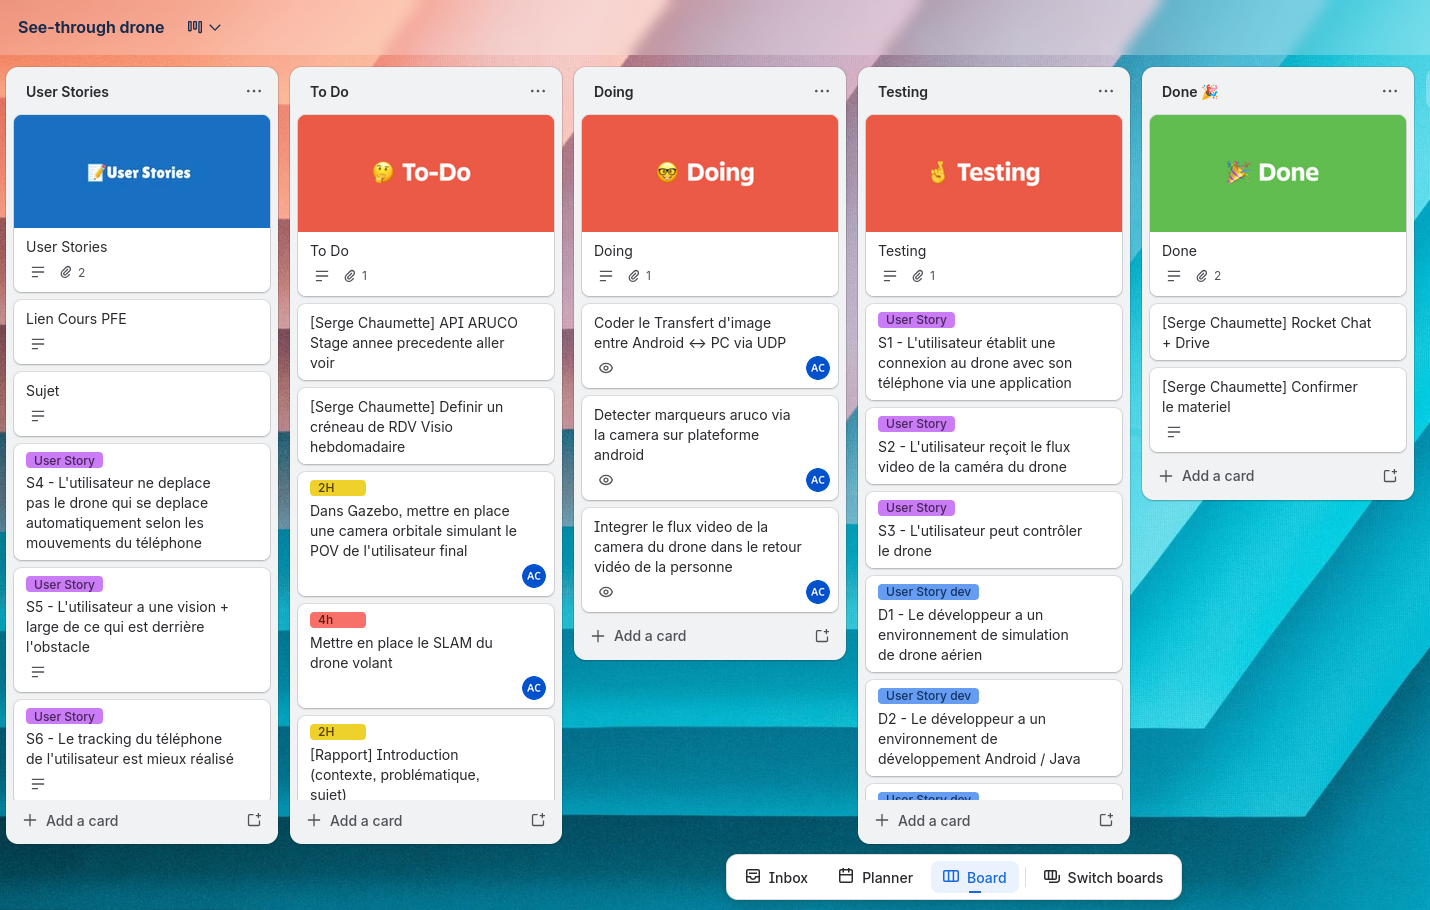
\includegraphics[width=0.7\linewidth]{img/trello.png}
    \caption{Aper\c cu du Kanban sur la plateforme Trello}
    \label{fig:placeholder}
\end{figure}

Cela est li\'e a la m\'ethodologie issue du cours de MOCPI avec les différents etapes de taches a completer

\section{Besoins}
Des besoins fonctionnels ont \'et\'e d\'egag\'es dans le cadre du projet.
\subsection{Fonctionnels}
\begin{itemize}
    \item Le système doit permettre la connexion entre le téléphone et le drone.
    \item Le système doit afficher le flux vidéo du drone.
    \item Le système doit permettre le contrôle du drone.
    \item Le système doit suivre la position du téléphone.
    \item Le système doit détecter des objets dans l’image.
    \item Le système doit afficher les éléments situés derrière un obstacle.
\end{itemize}
\subsection{Non Fonctionnels}
\begin{itemize}
    \item La latence du flux vidéo doit être inférieure à 200 ms.
    \item L’application doit fonctionner sur Android.
    \item Le système doit maintenir une connexion stable avec le drone.
    \item Le tracking doit être suffisamment précis pour maintenir la cohérence visuelle.
    \item L’interface doit être utilisable en temps réel.
\end{itemize}

\section{Choix logiciels}
Au cours de la r\'ealisation, des choix logiciels, de langages et de
biblioth\`eques ont du \^etre pris pour mener a bien le projet. Ici nous allons
discuter de ces choix et detailler notre raisonnement.
\subsection{Sur ordinateur}
La partie logiciel sur ordinateur a deux r\^oles principaux: Recevoir les donn\'ees de
capteurs du drone, et communiquer ces donnees avec le mobile de l'utilisateur.
En vue de communiquer avec le drone, nous avons fait le choix d'utiliser la
plateforme ROS. Il y a plusieurs raisons qui ont motiv\'e ce choix:
\begin{description}
    \item[Mod\`ele asynchrone fiable] ROS a un mod\`ele centr\'e sur une
    communication de messages via des topics. Ces messages fonctionnent via un syst\`eme de publisher/subscripter. Ce m\'echanisme permet de programmer des services s'executant de mani\`ere parall\`ele, sans se soucier de probl\'ematiques d'acc\`es concurrents.
    \item[Nombreuses bibliot\`eques] ROS est un ecosyst\`eme mature qui propose
    de nombreuses biblioth\`ques pertinentes pour le projet. Par exemple, le
    controle du drone via clavier a directement \'et\'e r\'ecup\'er\'e via
    \textit{teleop\_twist\_keyboard}. On profite aussi de types de messages standard a propager entre les services.
    \item[Choix de drone flexible] Tout drone qui implemente des drivers ROS
    devient compatible avec notre projet avec un minimum d'effort
    d'impl\'ementation a fournir.
    \item[Simulateur Gazebo] Choisir ROS permet d'utiliser le simulateur Gazebo, qui permet de simuler les donn\'es du drones et acc\'el\`ere le prototypage de nos services
\end{description}
ROS offre donc de nombreux avantages dans le cadre du projet. Pour son
int\'egration sur la machine, nous avons fait le choix de l'integrer via
conteneur (Docker). Cela est du au fait que certaines versions de ROS
requi\`erent une version pr\'ecise d'Ubuntu, et permet aussi de controler
pr\'ecis\'ement la version des d\'ependances syst\`emes (python, paquets pip
globaux, rosdep...) Les services ROS peuvent \^etre programm\'es en C++ ou en
python. Pour les services que nous avons programm\'e nous avons choisi python
pour la simplicit\'e de prototypage.
Toute la communication avec le drone a \'et\'e faite avec le paquet tello-ros2\cite{telloros}, qui utilise djitellopy\cite{djitellopy} pour r\'ecuperer les donn\'ees d'odom\'etries et contr\^oler le drone.

\subsection{Sur mobile}
La partie mobile de l'application a plusieurs r\^oles: Afficher un flux video a
l'utilisateur, r\'ecup\'erer les donnes de capteurs,traiter l'image, communiquer
avec la station fixe. Les options r\'epondant aux besoins sont assez restraintes sur
mobile, nous avons choisi de produire une application android native, en Java.
Ce choix permet d'utiliser les api android pour recup\'erer les donn\'ees de
capteurs(cam\'era, gyroscope...) mais demandera un certain effort
d'impl\'ementation si un jour on veut faire passer l'application vers IOS ou
bien des lunettes AR. Ce choix permet d'utiliser la biblioth\`que de Computer
Vision OpenCV pour traiter l'image, ce qui permet de s'appuyer sur les
comp\'etences vues au cours de l'ann\'ee.

\section{Architecture}

Pour r\'epondre aux besoins identifi\'es, nous avons mis en place une
architecture distribu\'ee avec 3 composants: le drone, le mobile de
l'utilisateur et le PC ex\'ecutant ROS.
Les \'el\'ements mat\'eriels du projet sont les suivants:
\begin{itemize}
    \item Drone DJI Tello EDU: Version educative du DJI Tello, qui expose plus d'api et permet de recuperer de nombreuses donn\'ees de capteurs. Il dispose d'une camera 720p qui diffuse 30 images par secondes.
    \item Pc portable: d'un point de vue mat\'eriel, il faut que le pc soit capable d'\'executer Docker, et qu'il dispose d'une carte wifi.
    Pour faire tourner la simulation Gazebo, il faut que le processeur de l'ordinateur ne soit pas trop faible, mais il est tol\'erable de ne pas faire tourner la simulation a 100\% de vitesse dans notre cas d'usage.
    \item Smartphone/Tablette Android: L'appareil doit avoir Android minimum version 7 pour \'ex\'ecuter l'application. Il est n\'ecessaire qu'il dispose d'une cam\'era.
\end{itemize}

Le sch\'ema suivant illustre l'architecture et les flux de donn\'ees principaux.
\begin{figure}
    \centering
    %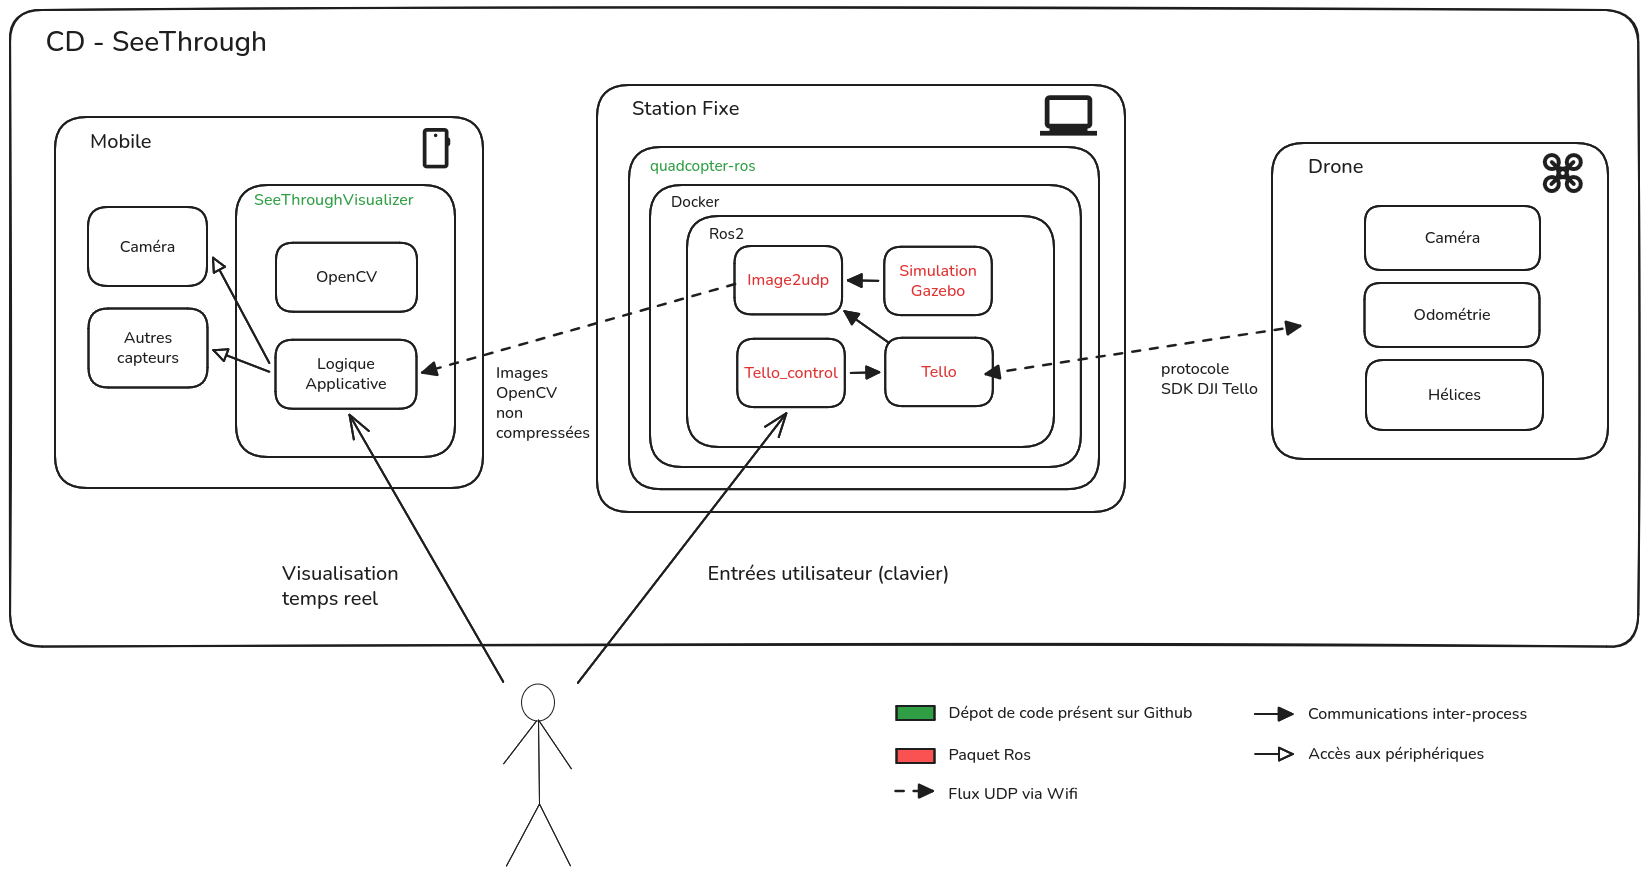
\includegraphics[width=0.7\linewidth]{img/architecture.png}
    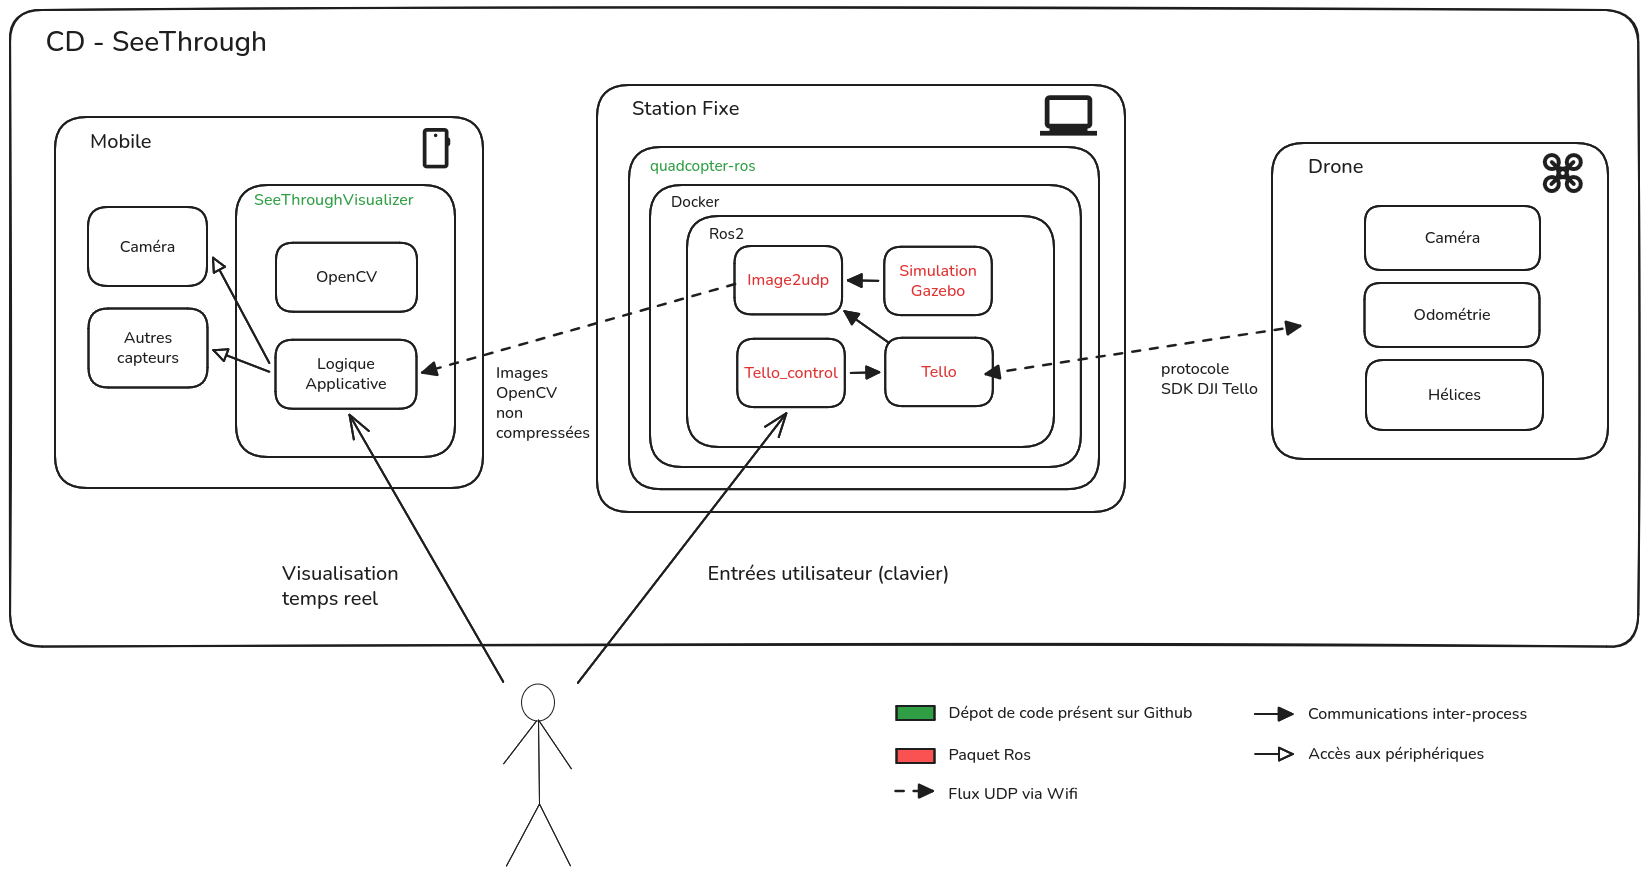
\includegraphics[width=1\linewidth]{img/architecture.png}
    \caption{Architecture CD-See-Through}
    \label{fig:placeholder}
\end{figure}
Nous allons ensuite d\'ecrire cette architecture plus en d\'etail en commen\c cant par les flux de donn\'ees.

\subsection{Flux de donn\'ees}
Le syst\`eme repose sur des \'echanges de donn\'ees entre le drone, l'appareil mobile et la station fixe (PC). 
D'un point de vue concret, pour que tous les \'el\'ements puissent communiquer,
on suit ce fonctionnement: Lorsque l'on allume le Tello, il diffuse un reseau,
le PC se connecte a ce r\'eseau. Ensuite, on doit configurer un point d'acc\`es
a acc\'eder sur le tello, par exemple le point d'acc\`es mobile du
t\'el\'ephone, puis le tello red\'emarre, et garde cette configuration en
m\'emoire. On connecte ensuite le PC au r\'eseau du mobile. En suivant
ce proc\'ed\'e, les trois appareils peuvent s'envoyer des messages r\'eseau. Une
fois connect\'es, le flux de donn\'ees est le suivant:

\begin{enumerate}
    \item Le drone transmet son flux video et ses donn\'ees de capteurs vers le pc via UDP, en suivant le protocole d\'ecrit dans le SDK DJI Tello\cite{tellosdk}.
    \item Le pc r\'ecup\`ere ces donnees, convertit l'image Ros en image OpenCV, puis les envoie vers le t\'el\'ephone non compress\'e via un flux UDP
    \item Le t\'elephone re\c coit le flux video du drone.
\end{enumerate}

\subsection{Station Fixe - Module ROS}
Comme indiqu\'e dans la partie choix logiciels, le code sous ROS s'articule sous
forme de paquets, chaque paquet a ensuite diff\'erents services, qui vont pour
certains venir attendre une entree utilisateur pour effectuer une
action/produire un message vers un autre topic ROS. D'autres services n'agissent
que lorsqu'ils re\c coivent un message a un certain topic. Ces services ROS sont
disponibles dans le d\'ep\^ot Github quadcopter-ros\cite{quadcopter_ros} dans le r\'epertoire
\textit{ros2\_ws/src}. L'objectif de la partie ROS est de collecter les donnees
du drone, les convertir dans un format adapt\'e, puis d'envoyer un flux vid\'eo
a l'appareil mobile.
On explique ensuite comment cela se concr\'etise dans notre environnement de travail ROS.

\subsubsection{ros\_gz\_*}
Les paquets ros\_gz\_application, ros\_gz\_bringup, ros\_gz\_description, et
ros\_gz\_gazebo sont tous des paquets relatifs au simulateur Gazebo.
\begin{description}
    \item[ros\_gz\_bringup] Fait le pont entre la nouvelle version de Gazebo et ROS.
    En effet Gazebo a ses propres topics, on \'ecrit ici l'equivalent ros du topic Gazebo, cela permet de recevoir les informations de capteurs simul\'es
    \item[ros\_gz\_description] Contient les descriptions des diff\'erents fichiers de mod\`eles. C'est ici que nous avons ajout\'e le mod\`ele du quadricopt\`ere par exemple.
    \item[ros\_gz\_gazebo] Contient le code utilis\'e pour faire tourner la simulation Gazebo(pas modifi\'e dans le projet)
\end{description}

\subsubsection{tello}
Les paquets tello, tello\_msg et tello\_control proviennent tous du paquet ROS
cit\'e pr\'ec\'ecedemment: tello-ros2i\cite{telloros}. Ce paquet permet
d'obtenir des messages ROS a partir de DJITelloPY. 
Le paquet tello est les paquet central qui produit les messages.
Le paquet tello\_msg est seulement un type de message utilis\'e par tello.
Enfin le paquet tello\_control permet de controller le drone a l'aide du clavier.

\subsubsection{image2udp}
Ce paquet a été développé dans le cadre du projet. Il permet de convertir les
images issues des messages ROS (type \texttt{sensor\_msgs/Image}) en format
exploitable par OpenCV, puis de transmettre ces images vers le dispositif mobile
via le protocole UDP.

\subsection{Appareil Mobile - Module Android}
Le module Android est l'interface principale de l'utilisateur avec
l'application. Son objectif est de retranscrire est d'afficher le flux video de
l'utilisateur, et de remplacer une detection de l'obstacle par le flux video du
drone.
Pour r\'epondre a ce besoin, nous avons mis en place une application native Android\cite{seethroughvisualizer}, dans laquelle nous avons integr\'e OpenCV pour effectuer le traitement de l'image.
Cette application est constitu\'ee de trois classes:
\begin{description}
    \item[UdpVideoReceiver] Re\c coit le flux UDP de ROS, et le convertit au format OpenCV Matrice.
    \item[Vision]Diff\'erentes fonctions de d\'etection/traitement sur image.
    \item[MainActivity] Instancie les diff\'erents \'el\'ements de l'interface 
    et appelle les fonctions des autres classes pour presenter la vue camera a l'utilisateur.
\end{description}

\section{Réalisation}
Au cours du projets, nous avons d\'evelopp\'e deux solutions sur deux plateformes diff\'erentes, dont nous allons d\'etailler le d\'eveloppement ainsi que le fonctionnement lors de cette partie.
\subsection{Simulation Gazebo}
Au d\'ebut du projet, il a \'et\'e d\'ecid\'e d'utiliser l'environnement de simulation Gazebo avec ROS. En effet cela a permis de commencer a programmer la partie ROS sans forc\'ement avoir le mat\'eriel.
Pour utiliser la plateforme ROS, un script de lancement Docker a \'et\'e mis en place, qui installe les d\'ependances requises, et utilise les bonnes options Docker pour voir le r\'eseau de la machine h\^ote ainsi que faire passer les fenetres graphiques.
La base du code et l'int\'egration ROS avec Gazebo se base sur un template disponible dans la documentation de Gazebo\cite{templategazebo}.
Une fois la base de la simulation fonctionnelle, nous avons mis en place un environnement minimal dans Gazebo, permettant de d\'evelopper la suite du projet.
L'image suivante montre cet environnement.
\begin{figure} [H]
    \centering
    %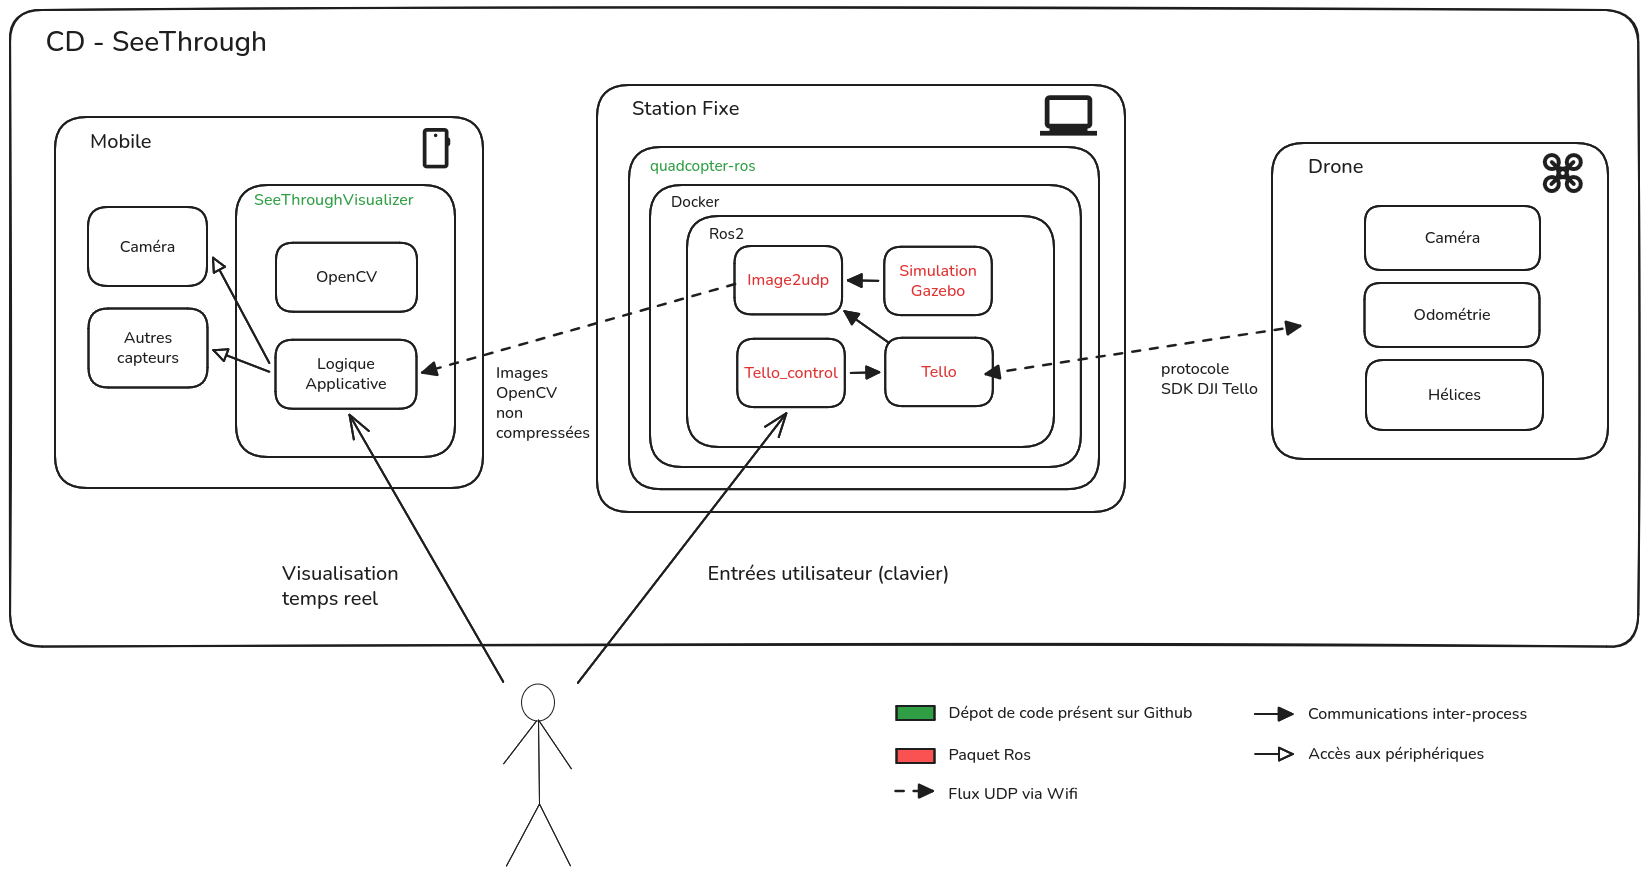
\includegraphics[width=0.7\linewidth]{img/architecture.png}
    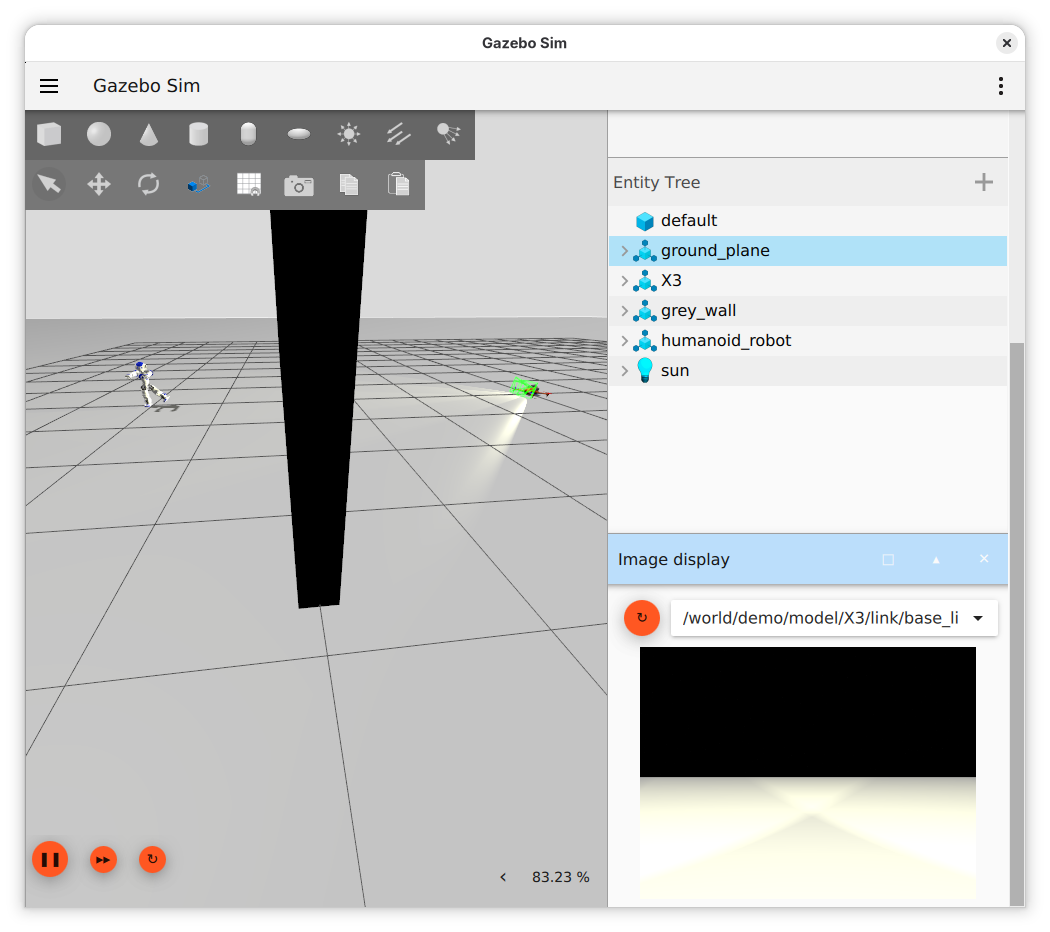
\includegraphics[width=0.7\linewidth]{img/gazebo.png}
    \caption{Environnement de simulation Gazebo}
    \label{fig:placeholder}
\end{figure}
Cet environnement est constitu\'e d'un drone quadricopt\`ere, faisant face a un mur, avec de l'autre c\^ot\'e un robot humanoide. Dans le coin droit, on observe le flux vid\'eo de la cam\'era du drone simul\'e.
Le monde de la Simulation Gazebo est d\'ecrit via un fichier sdf (format de ficher propre a Gazebo sous format XML), dont voici un extrait du monde suivant:

\begin{lstlisting}[language=Xml, caption= Description du monde Gazebo]
<?xml version="1.0" ?>
<sdf version="1.8">
  <world name="demo">
    <plugin
      filename="gz-sim-physics-system"
      name="gz::sim::systems::Physics">
    </plugin>
    <!-- ...
        plugins de la simulation Gazebo
    -->

    <light name="sun" type="directional">
      <cast_shadows>true</cast_shadows>
      <pose>0 0 10 0 0 0</pose>
    </light>

    <model name="ground_plane">
      <static>true</static>
      <link name="link">
        <collision name="collision">
          <geometry>
            <plane>
              <normal>0 0 1</normal>
              <size>100 100</size>
            </plane>
          </geometry>
        </collision>
        <!-- ... -->
    </model>

    <!-- Modele du drone -->
    <model name="X3">
      <self_collide>true</self_collide>
      <pose>0 0 0.35 0 0 0</pose>
      <include merge="true">
        <uri>package://ros_gz_description/models/X3</uri>
        <plugin
        filename="gz-sim-multicopter-motor-model-system"
        name="gz::sim::systems::MulticopterMotorModel">
        </plugin>
    </model>
    <!-- Nombreux plugins odometrie capteurs omis.. -->

    <!-- Modele du mur -->
    <model name="grey_wall">
      <self_collide>true</self_collide>
      <pose>4.00 0 0 0 0 1.57</pose>
    <!-- ... -->
    </model>
    
    <!-- Modele du robot humanoide -->
    <model name="humanoid_robot">
      <self_collide>true</self_collide>
      <pose>6.00 0 0 0 0 1.57</pose>
      <!-- ... -->
    </model>
  </world>
</sdf>
\end{lstlisting}

Concr\`etement l'int\'eret de la simulation dans le cadre du projet est
l'extraction d'un flux vid\'eo ROS de type similaire a celui qui est re\c cu
avec le drone r\'eel, ce qui est utilis\'e comme base pour implementer la suite du projet. 

\begin{lstlisting}[caption= Conversion du topic Gazebo vers Ros dans
quadcopter-ros/ros2\_ws/src/ros\_gz\_bringup/config/ros\_gz\_X3\_bridge.yaml]
- ros_topic_name: "camera/camera_image"
  gz_topic_name: "/world/demo/model/X3/link/base_link/sensor/camera_front/image"
  ros_type_name: "sensor_msgs/msg/Image"
  gz_type_name: "gz.msgs.Image"
\end{lstlisting}

Le code yaml precedent indique qu'il faut convertir les messages du topic
Gazebo(l'image de la video du drone simul\'e) vers le topic ROS
\texttt{/camera/camera\_image}).

Les \'el\'ements de physique et m\'eme la detection d'aruco ne sont pas
impl\'ementes dans la simulation. Certains \'el\'ements ont \'et\'e commenc\'es mais pas finis car demande beaucoup de code pour etre mis en place (ex: le robot humanoide).
Les efforts de d\'eveloppement ont \'et\'e redirig\'es vers l'imple\'ementation sur le drone concret une fois qu'il a \'et\'e re\c cu.

\subsection{Integration de l'API du drone}
Une fois le mod\`ele du drone confirm\'e et apr\`s sa r\'eception, nous avons pu commencer a travailler a son integration dans l'environnement ROS.
D'abord, nous avons voulu confirmer le fonctionnement de celui ci en utilisant l'appli DJI Tello\cite{djitellopy}

\begin{figure}
    \centering
    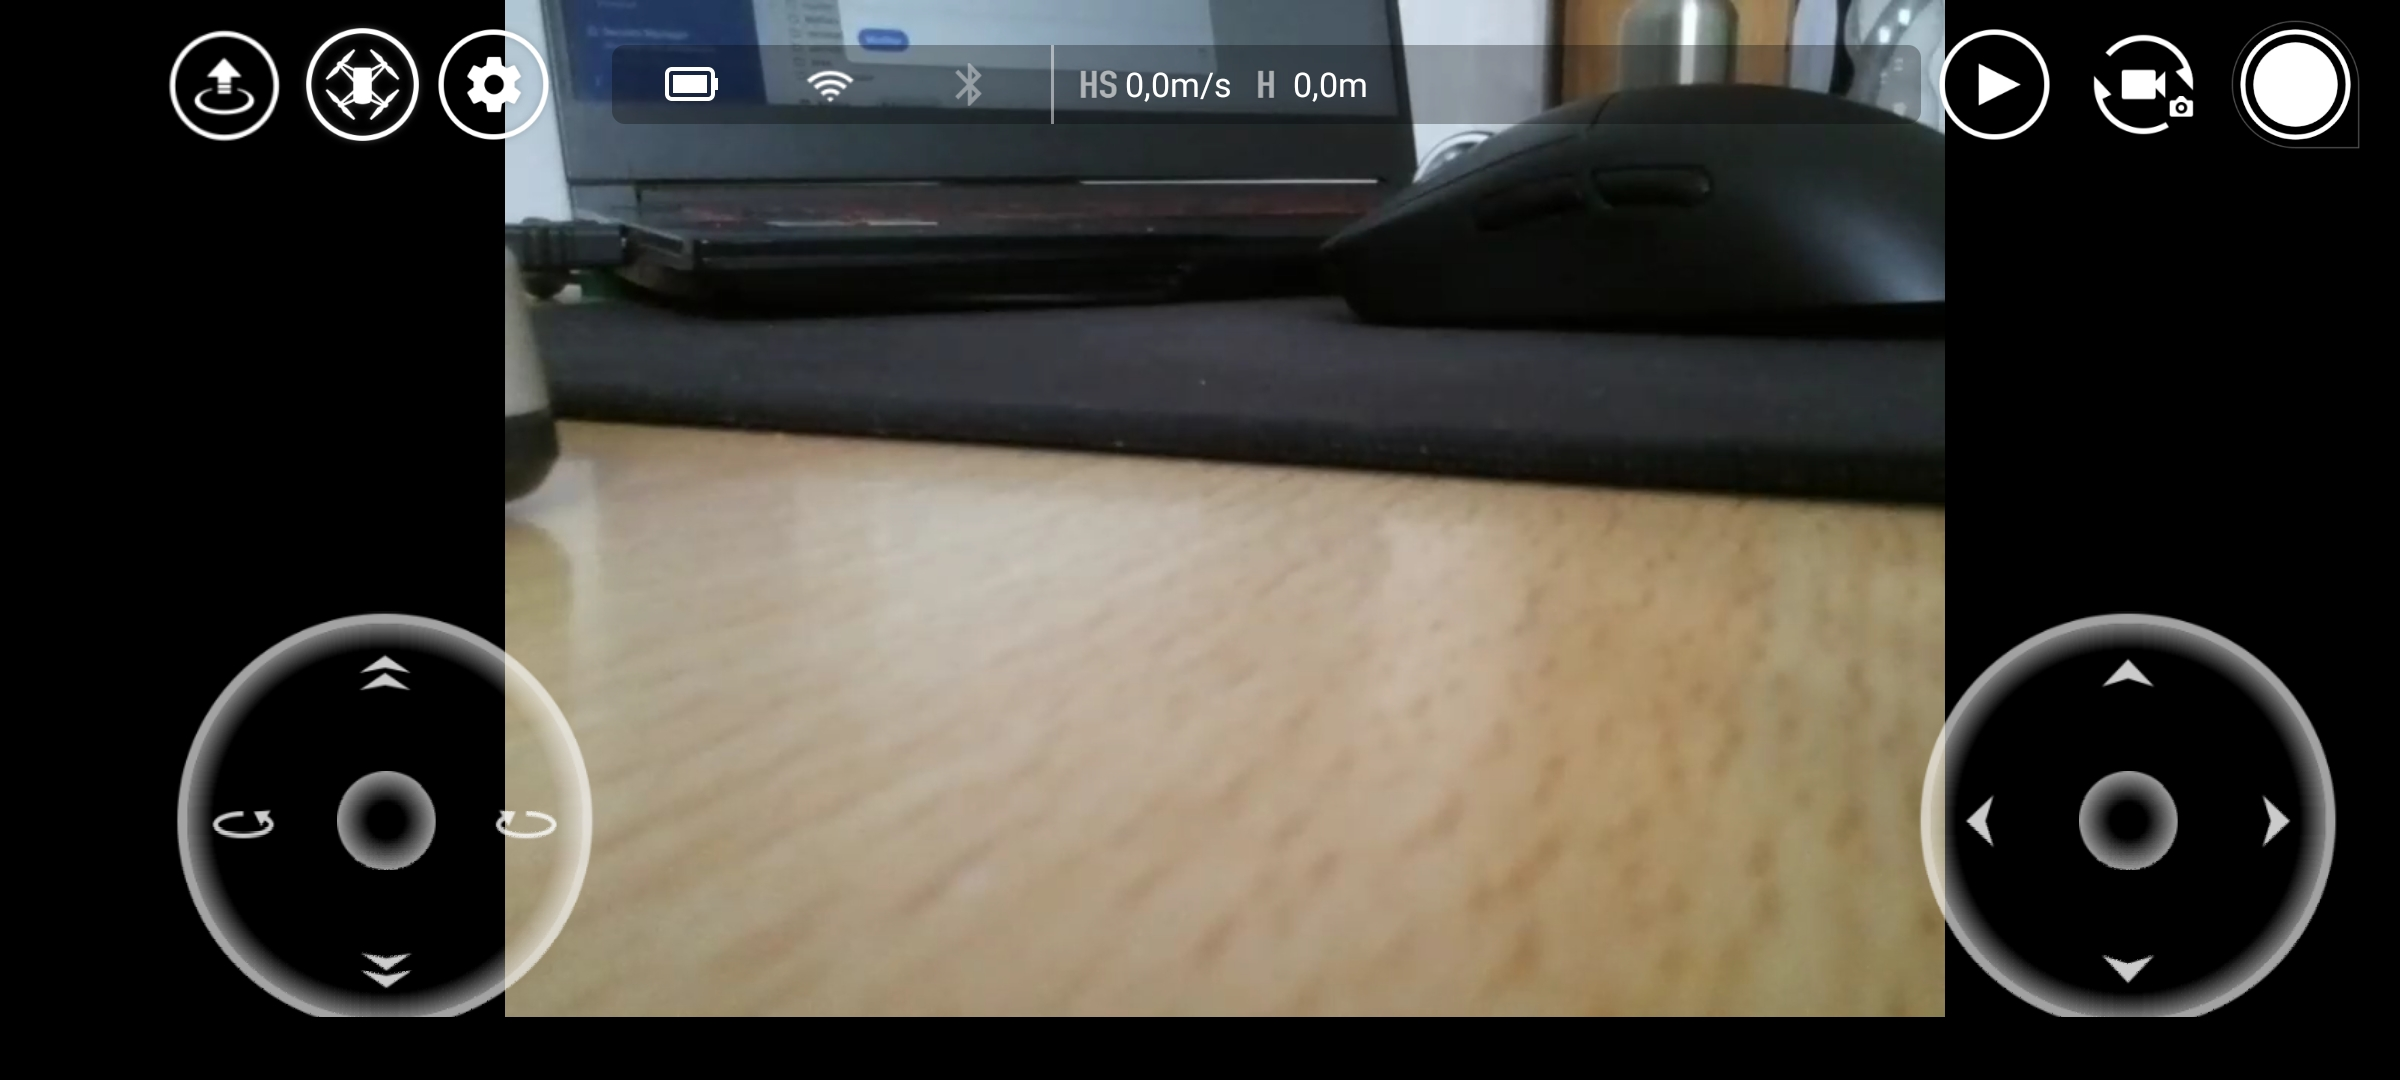
\includegraphics[width=0.7\linewidth]{img/dji_tello_app.jpg}
    \caption{Interface de l'application DJI Tello connect\'ee au drone}
    \label{fig:placeholder}
\end{figure}

Grace a cette application, nous avons pu confirmer la connection au drone et que les diff\'erents \'elements soient fonctionnels (d\'ecollage, controle, flux video...).

Nous avons ensuite travaill\'e a l'integration du drone dans l'environnement ROS.
Comme expliqu\'e dans la partie architecture, un module ROS a \'et\'e trouv\'e
en ligne\cite{telloros} et impl\'emente directement les diff\'erentes
fonctionnalit\'es dont nous avons besoin pour la suite du projet.

\begin{figure}
    \centering
    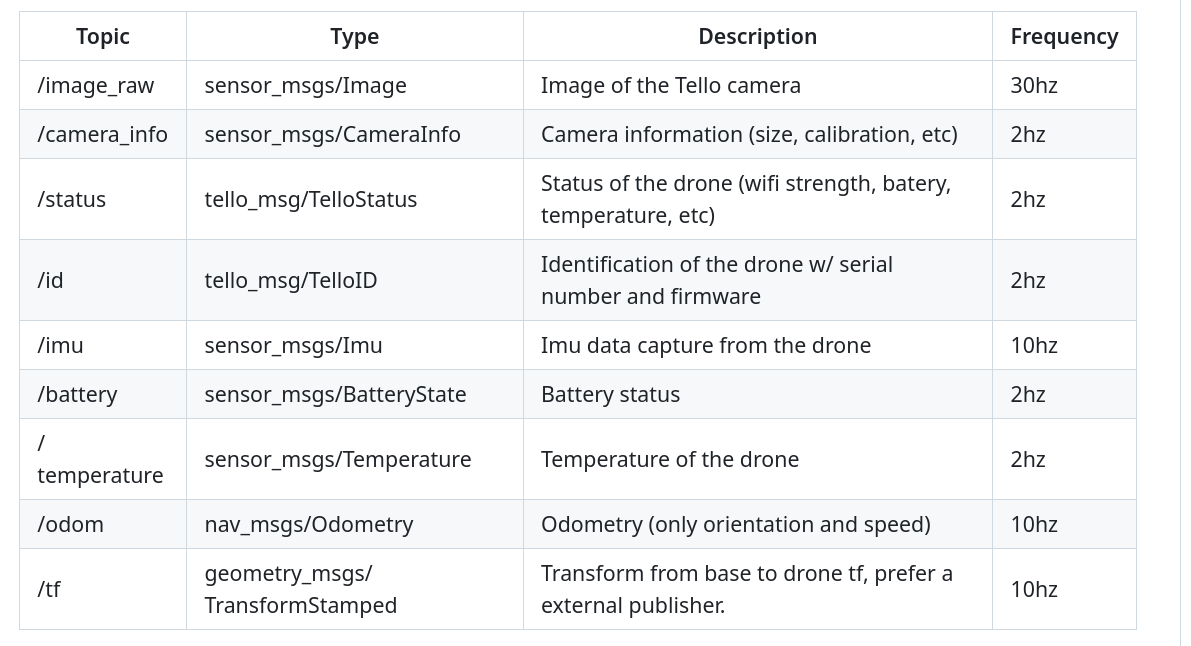
\includegraphics[width=1\linewidth]{img/telloros_topics.png}
    \caption{Liste des messages et leurs topics publi\'es par tello\_ros2}
    \label{fig:placeholder}
\end{figure}

Apr\`es avoir ajout\'e le paquet Ros, install\'e les diff\'erentes d\'ependances, il suffit de lancer la node principale, en ayant le drone connect\'e au r\'eseau pour avoir acc\`es aux messages des topics list\'es  dans la capture d'\'ecran.
Le message qui nous int\'eresses est l'image au topic \textit{/image\_raw}.
A noter que de base le drone se met en "access point", ce qui signifie qu'il
agit comme un point d'access wifi vers les autres hotes. Nous avons modifi\'e la
methode utilisee dans le package tello pour pouvoir modifier ce mode et le
mettre en mode "station", ce qui permet d'assigner le drone sur notre r\'eseau.

\begin{figure}
    \centering
    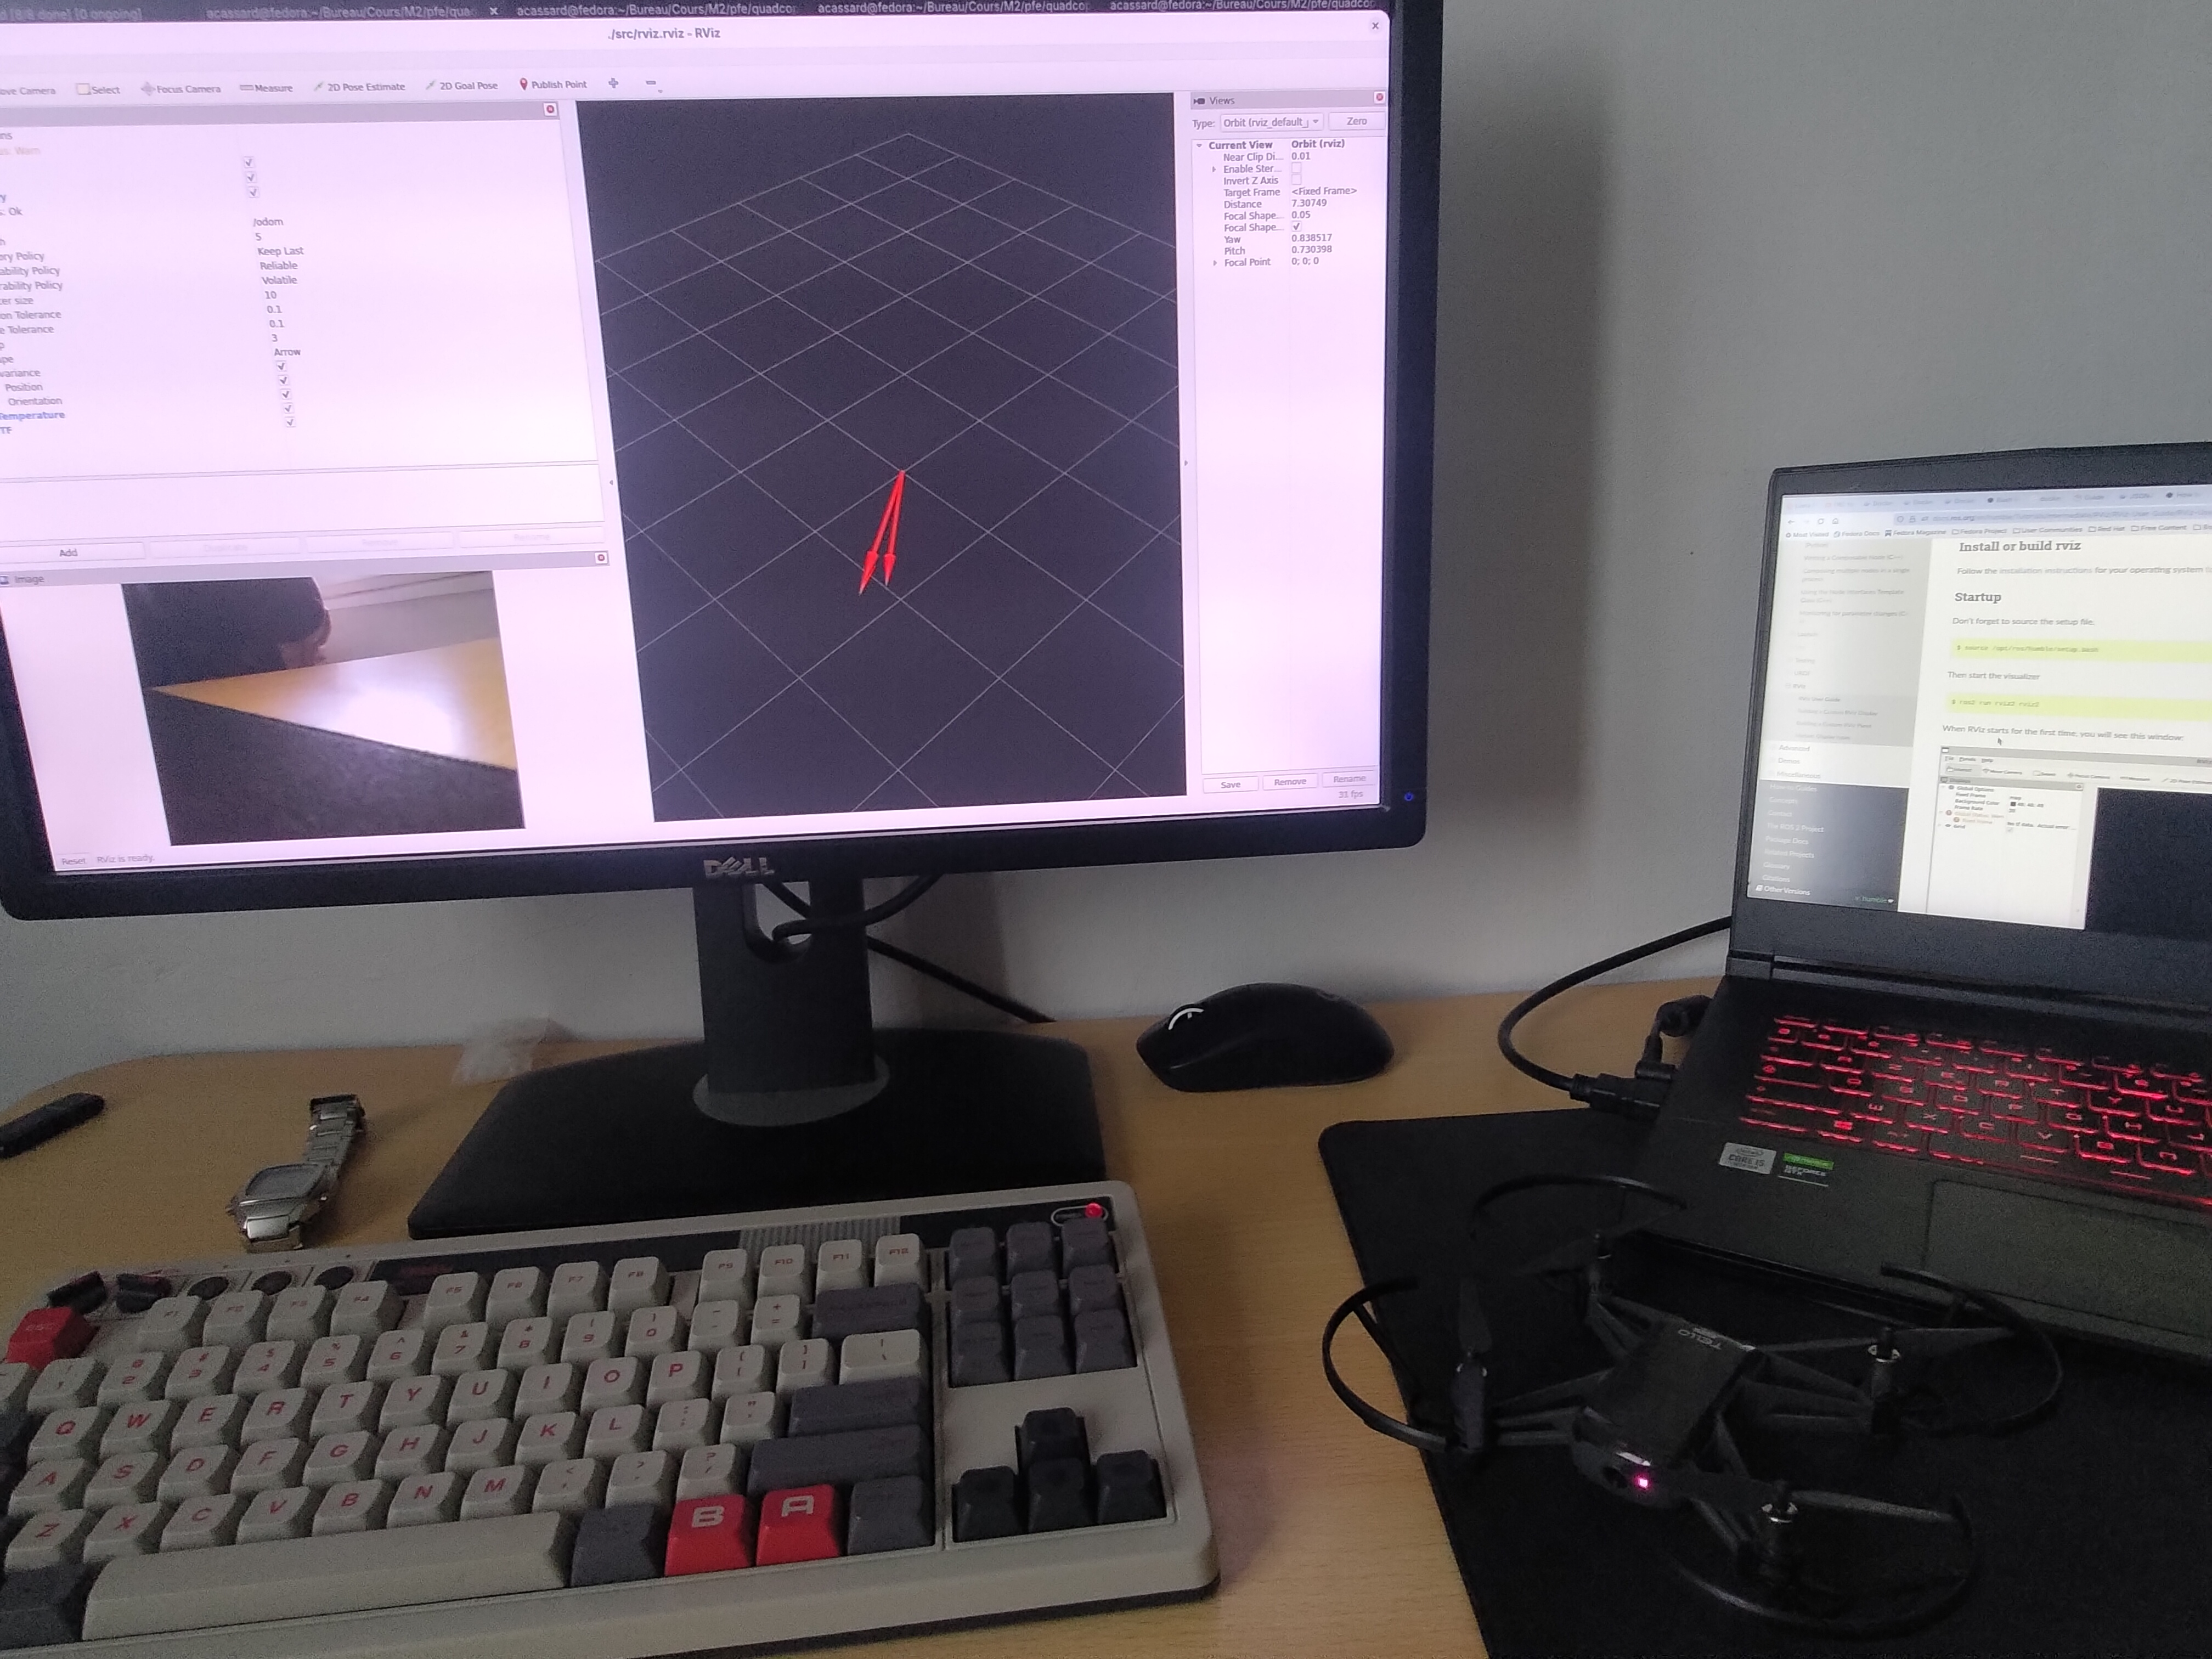
\includegraphics[width=1\linewidth]{img/rviz_tello.jpg}
    \caption{Connexion a la Node tello et acces au flux camera / odometrie via ROS}
    \label{fig:placeholder}
\end{figure}

\subsection{image2udp}
Une fois que nous re\c cevons le flux video du drone vers ROS, le d'efi est
d'envoyer ce flux vers l'appareil android. Le plan initial \'etait d'envoyer
directement un flux vid\'eo via RTSP(protocole d'envoi de video via TCP/UDP) au
telephone. La partie ROS de ce type d'envoi \'etait fonctionnel, mais pas la
partie Android, qui necessite un d\'ecodage qui n'etait pas int\'egr\'e dans la
version d'OpenCV int\'egr\'ee au projet Android. Apr\`es avoir essay\'e
diff\'erent moyens de d\'ecoder ce flux (linkage de FFMPEG arm au projet opencv,
ouverture via librairie Media avec code natif android...) Il a \'et\'e
d\'ecid\'e d'envoyer l'image de maniere plus simple: envoyer directement les
donn\'es de l'image via UDP. Un camarade du projet CD Suspension System
(Anthonin Brauer) avait d\'ej\'a fait face a la meme prob\'ematique et avait
deja cod\'e l'envoi et la r\'eception d'images OpenCV via Python. 
Nous lui avons donc demand\'e la permission de reutiliser son code dans notre
projet. Il a accept\'e, et il s'av\`ere que son code fonctionne bien.
Le travail a donc \'et\'e de convertir son code d'envoi. 
En effet dans son projet il transf\`ere de client python a client python mais nous voulons transf\'erer ici de client python(img Ros) a client Java.
Le code d'Anthonin d\'ecoupe les images en bloc de 60 000 bytes maximum et les
envoie avec des Headers indiquant les id de frame, ainsi que potentiellement un
id de chunk. 

\begin{lstlisting}[language=Python, caption= d\'ecoupe des images en morceaux a envoyer sur le r\'esau dans UdpVideoService]
chunk_count = (payload_len + MAX_CHUNK_SIZE - 1) // MAX_CHUNK_SIZE
if chunk_count > 65_535:
    print("WARNING: image too large even for chunked transfer")
    return

current_frame_id = self.frame_id
self.frame_id = (self.frame_id + 1)

for chunk_idx in range(chunk_count):
    start = chunk_idx * MAX_CHUNK_SIZE
    end = min(start + MAX_CHUNK_SIZE, payload_len)
    chunk = payload_bytes[start:end]
    header = struct.pack(HEADER_FORMAT, current_frame_id, chunk_count, chunk_idx)
    packet = header + chunk
    try:
        self.sock.sendto(packet, (self.host, self.port))
    except:
        pass
\end{lstlisting}

Nous prenons donc les images issues de notre topic Ros (\textit{/image\_raw} pour le vrai drone ou \textit{/camera/camera\_image} pour l'image de la simulation), nous convertissons ces images au format OpenCV, puis on les envoie a l'adresse de l'appareil Android cible.

\begin{lstlisting}[language=Python, caption= Image2udp convertit et envoie l'image par Udp]
class Image2udp(Node):

    def __init__(self):
        super().__init__('minimal_subscriber')
        self.subscription = self.create_subscription(
            Image,
            '/camera/camera_image', # Ici le topic de la simu
            self.listener_callback,
            10)
        self.subscription  # prevent unused variable warning
        self.bridge = CvBridge()
        self.video_service = UdpVideoService(host="192.168.1.182")  # Phone's address

    def listener_callback(self, img_msg):
        cv_image = self.bridge.imgmsg_to_cv2(img_msg, desired_encoding='passthrough')
        self.video_service.send(cv_image)
\end{lstlisting}

Le code de listener\_callback s'execute a chaque fois que ROS recoit un message sur le topic indiqu\'e, donc a chaque image du drone.

\subsection{R\'eception du flux video sur Android}
La partie ROS mise en place, il a fallu s'occuper de la mise en place de la partie mobile principale interface de l'utilisateur.
D'abord il a fallu faire la r\'eciproque en java du code pr\'ecedent pour recevoir l'image UDP du r\'eseau.
Sur la plateforme Android, on peut pas utiliser des cv.imread comme en python sur pc fixe par exemple, il faut dire au Thread d'UI de venir peindre notre image Bitmap sur une case pr\'ed\'efinie de notre layout.

\begin{lstlisting}[language=Java,  caption=R\'ec\'eption de l'image ROS et affichage sur L'UI - UDPVideoReceiver.java]
            while (true) {
                DatagramPacket packet = new DatagramPacket(buffer, buffer.length);
                socket.receive(packet);

                int length = packet.getLength();
                long now = System.currentTimeMillis();

                if (length < HEADER_SIZE) continue;

                ByteBuffer header = ByteBuffer.wrap(packet.getData(), 0, HEADER_SIZE);
                header.order(ByteOrder.BIG_ENDIAN);

                int frameId = header.getInt();
                int chunkCount = header.getShort() & 0xFFFF;
                int chunkIdx = header.getShort() & 0xFFFF;

                byte[] chunk = new byte[length - HEADER_SIZE];
                System.arraycopy(packet.getData(), HEADER_SIZE, chunk, 0, chunk.length);

                FrameEntry entry = frames.get(frameId);
                if (entry == null) {
                    entry = new FrameEntry();
                    entry.total = chunkCount;
                    entry.updatedAt = now;
                    frames.put(frameId, entry);
                }

                entry.chunks.put(chunkIdx, chunk);
                entry.updatedAt = now;

                if (entry.chunks.size() != entry.total) {
                    // Cleanup stale frames
                    frames.entrySet().removeIf(e -> now - e.getValue().updatedAt > FRAME_TIMEOUT_MS);
                    continue;
                }

                // Reassemble frame
                int totalSize = 0;
                for (int i = 0; i < entry.total; i++) {
                    totalSize += entry.chunks.get(i).length;
                }

                byte[] assembled = new byte[totalSize];
                int offset = 0;
                for (int i = 0; i < entry.total; i++) {
                    byte[] c = entry.chunks.get(i);
                    System.arraycopy(c, 0, assembled, offset, c.length);
                    offset += c.length;
                }

                frames.remove(frameId);
                // Decode image using OpenCV
                Mat mat = Imgcodecs.imdecode(new Mat(1, assembled.length, org.opencv.core.CvType.CV_8U) {{ put(0,0,assembled); }}, Imgcodecs.IMREAD_COLOR);

                if (mat.empty()) continue;

                Bitmap bmp = Bitmap.createBitmap(mat.cols(), mat.rows(), Bitmap.Config.ARGB_8888);
                Utils.matToBitmap(mat, bmp);

                this.activity.runOnUiThread(() -> imageView.setImageBitmap(bmp));
            }
\end{lstlisting}

Une prem\`ere version de debug a etee teste\'ee: en haut, le flux de la cam\'era ouvert par openCV, en bas le flux re\c cu par la simulation.

\begin{figure}[H]
    \centering
    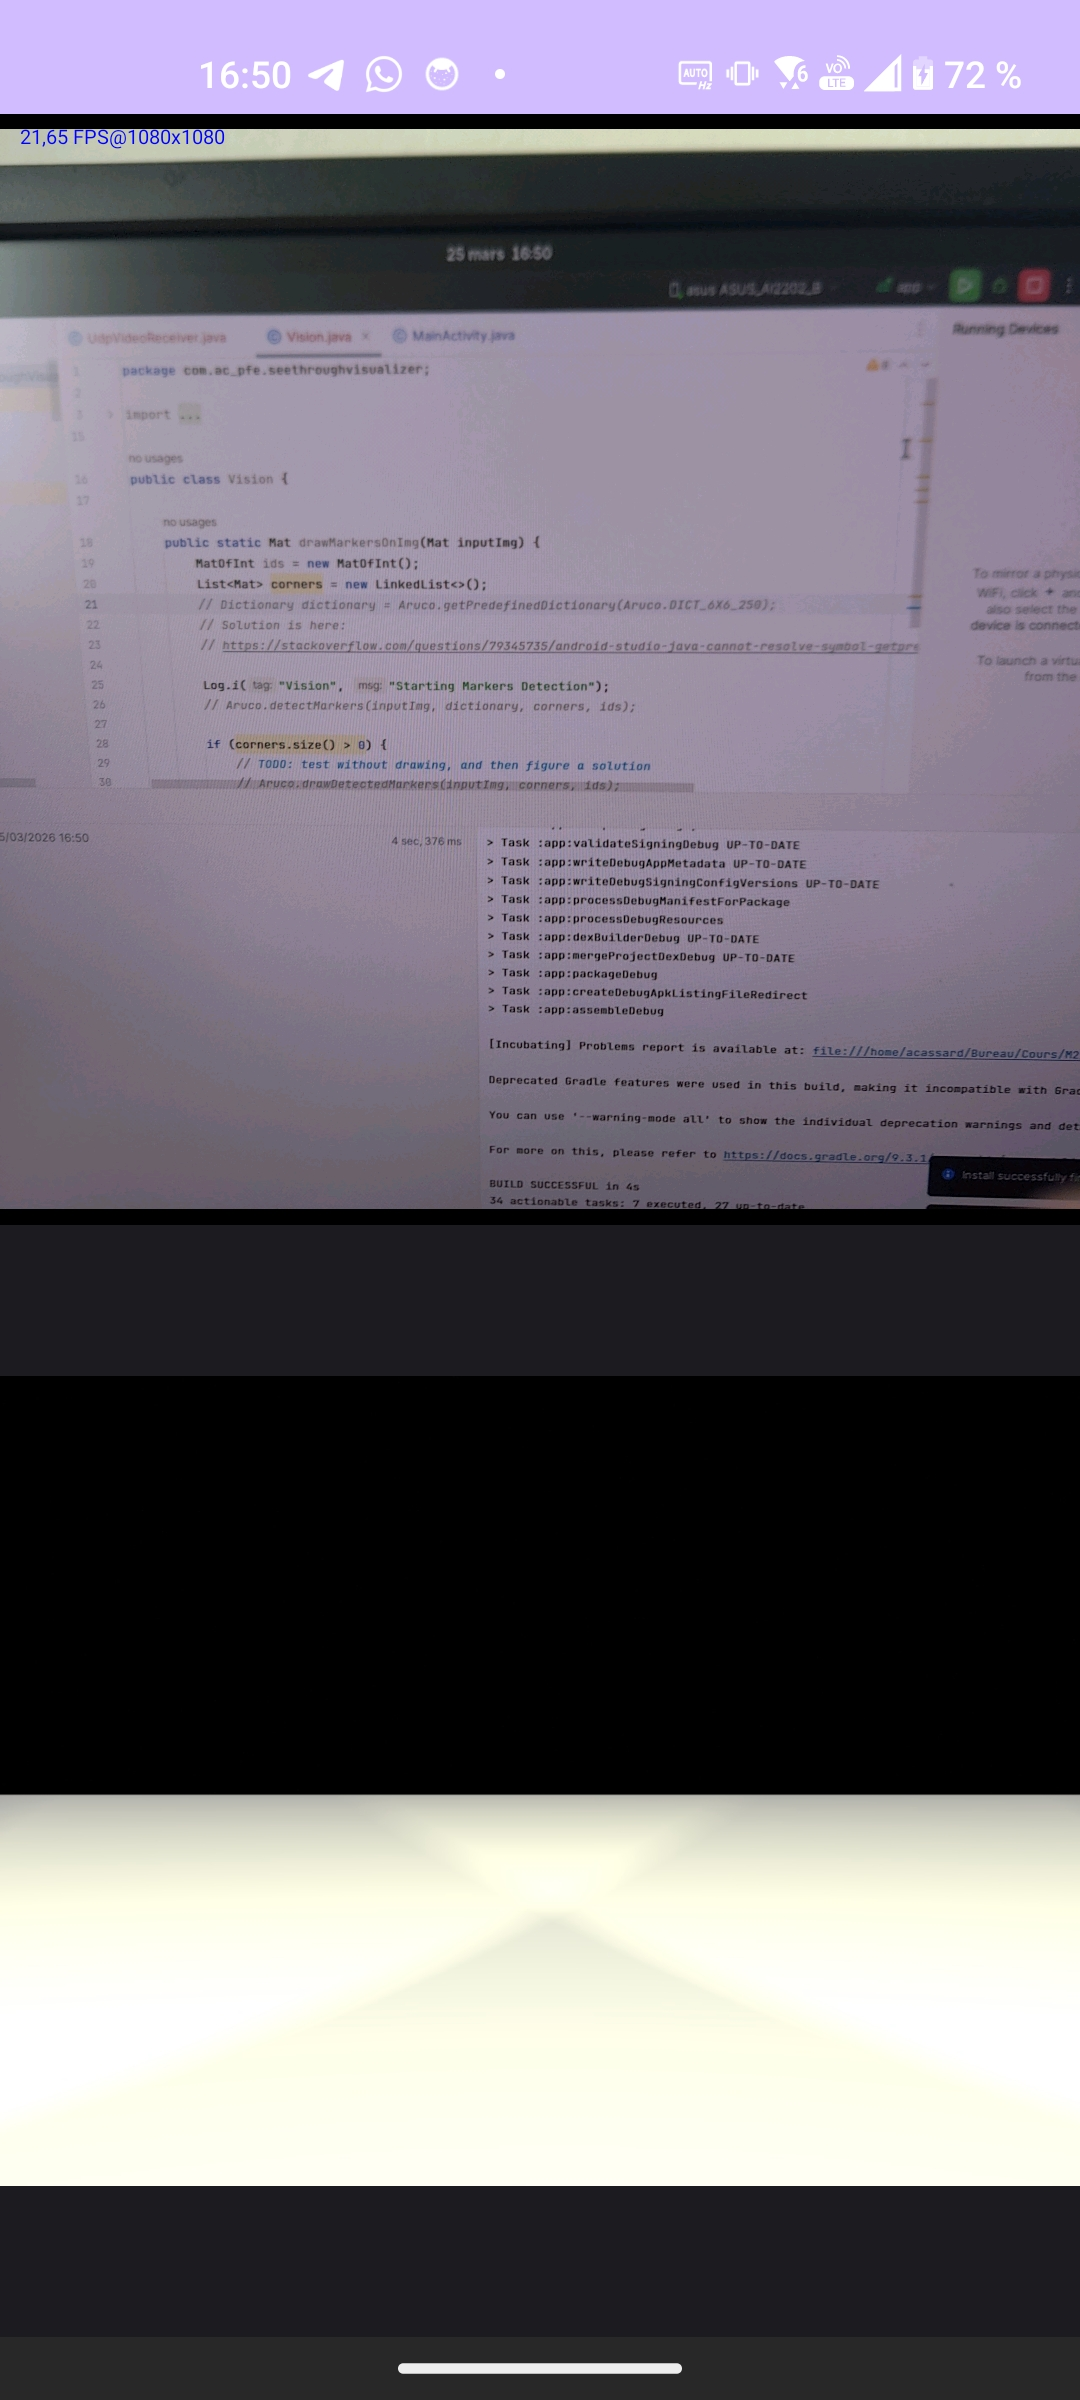
\includegraphics[width=0.7\linewidth]{img/SeeThroughVisualizer.jpg}
    \caption{Vue de debug de l'appli Android}
    \label{fig:placeholder}
\end{figure}

\subsection{D\'etection de planche ChArUco / Int\'egration dans l'image}

Pour r\'epresenter l'obstacle, l'utilisateur doit poser une planche ChArUco sur l'obstacle cible.
La g\'eneration de la planche ChArUco se situe dans le projet quadcopter-ros dans
\textit{aruco\_tools/generate\_charuco.py}.
Nous venons ensuite capturer l'image avec OpenCV, detecter la planche ChArUco, puis a partir des donn\'ees correspondantes, remplacer le rectangle dans l'image par le flux vid\'eo issu du drone.

\begin{figure}[H]
    \centering
    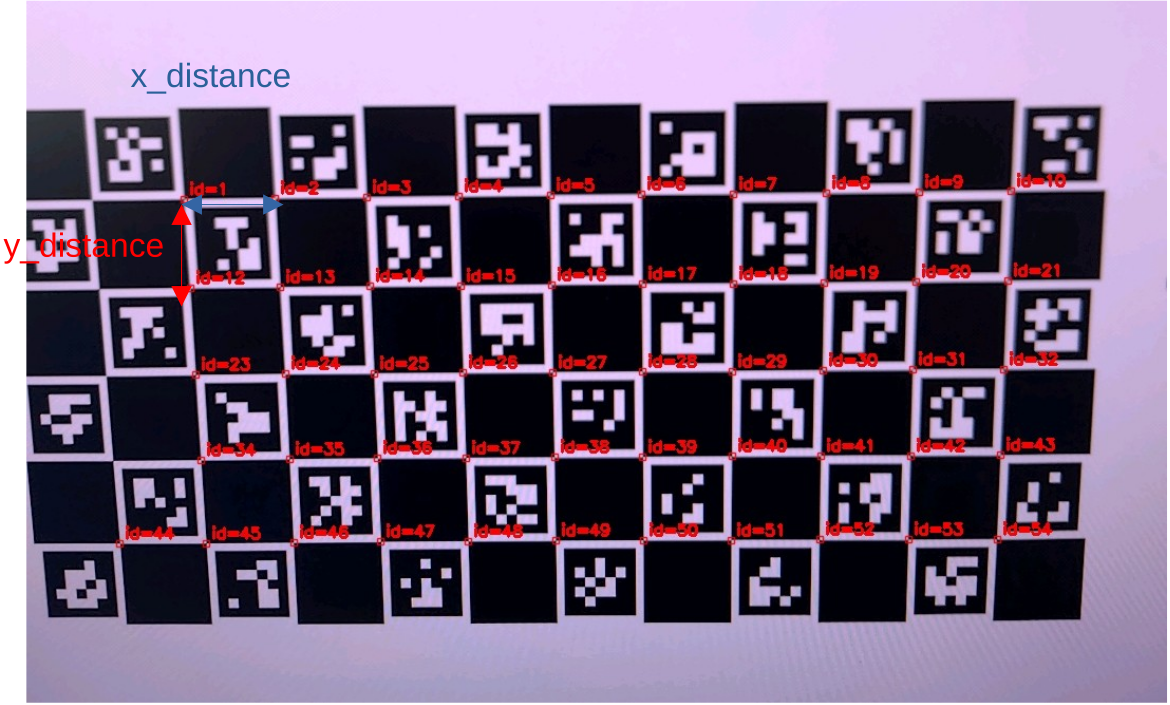
\includegraphics[width=0.7\linewidth]{img/charuco_ids.png}
    \caption{Detection des coins de la planche, avec leur id associ\'es}
    \label{fig:placeholder}
\end{figure}

Une fois les coins detect\'es, on selectionne un point d'ancrage, un point \'etant sur une colonne diff\'erente(x\_referent), un point \'etant sur une ligne diff\'erente(y\_referent). On utilise les coordoon\'ees des points pour determiner la distance entre deux carr\'es de la planche:

\begin{lstlisting}[language=Java,  caption=Calcul de la distance entre deux carr\'es sur l'image]
        for (int i = 0; i < charucoIds.rows(); i++) {
            Double idAsDouble = charucoIds.get(i,0)[0];
            // Position as square in the board
            int globalId = idAsDouble.intValue();
            // Index in the corners pos array
            int cornerId = i;
            int x = globalId % CHARUCO_COLS;
            int y = globalId / CHARUCO_COLS;

            if (anchor == null) {
                anchor = new int[]{globalId, cornerId, x, y};
            } else {
                // NOTE: it is possible that x_referent == y_referent
                // First corner that can give us x distance
                if (x_referent == null && anchor[2] != x) {
                    x_referent = new int[]{globalId, cornerId, x, y};
                }
                // First corner that can give us y distance
                if (y_referent == null && anchor[3] != y) {
                    y_referent = new int[]{globalId, cornerId, x, y};
                }
            }
        }
        // x distance between 2 squares in img pixels
        x_distance = Math.abs(x_referent_pos.x - anchor_pos.x) / Math.abs(x_referent[2] - anchor[2]);
        // y distance between 2 squares in img pixels
        y_distance = Math.abs(y_referent_pos.y - anchor_pos.y) / Math.abs(y_referent[3] - anchor[3]);
\end{lstlisting}

A partir de ces distances, on d\'etermine le coin haut a gauche, et le coin bas a droite.

\begin{lstlisting}[language=Java,  caption=Calcul de la position des coins de la planche]
Point top_left = new Point(anchor_pos.x - x_distance * (anchor[2] + 1), anchor_pos.y - y_distance * (anchor[3] + 1));
Point bottom_right = new Point(anchor_pos.x + x_distance * (CHARUCO_COLS - anchor[2] - 1), anchor_pos.y + y_distance * (CHARUCO_ROWS - anchor[3] - 1));
\end{lstlisting}

\begin{figure}[H]
    \centering
    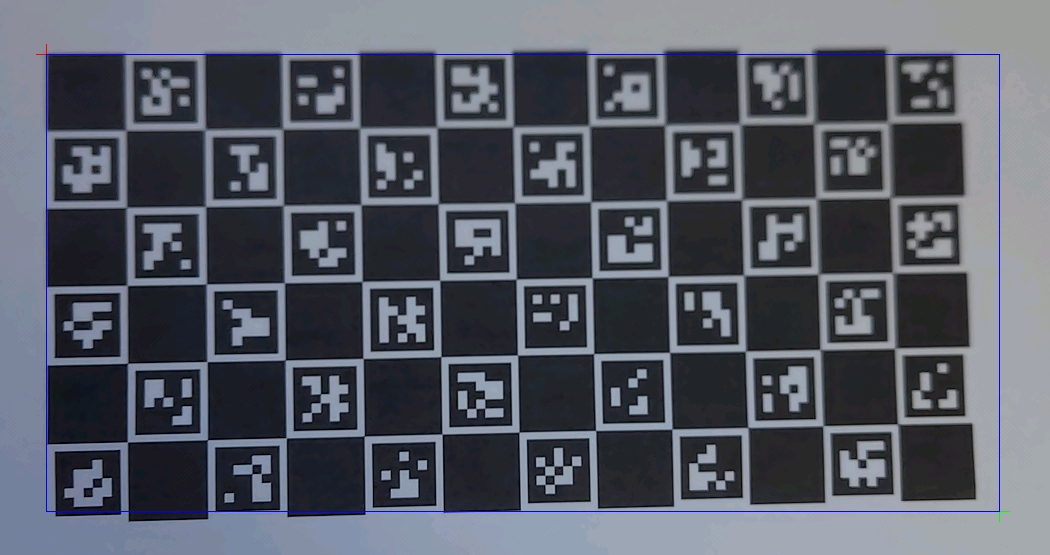
\includegraphics[width=0.7\linewidth]{img/rectangle_on_charuco.jpg}
    \caption{Dessin du rectangle form\'e par top\_left et bottom\_right}
    \label{fig:placeholder}
\end{figure}

On vient ensuite copier le contenu du flux vid\'eo re\c cu par udp dans ce rectangle.
\begin{figure}[H]
    \centering
    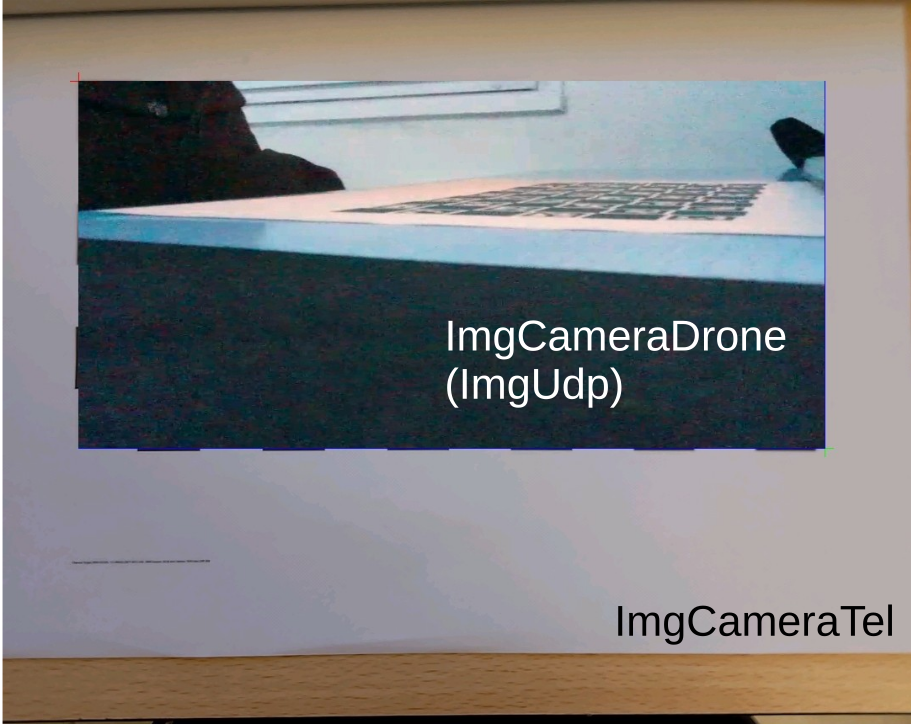
\includegraphics[width=0.7\linewidth]{img/see_through.png}
    \caption{Image du drone copi\'ee dans l'image du t\'el\'ephone}
    \label{fig:placeholder}
\end{figure}


\addcontentsline{toc}{section}{\protect Bilan}
\subsection*{Bilan}
A la fin du projet, on constate que beaucoup de compromis ont du \^etre faits par rapport a la vision initiale.
\begin{itemize}
    \item Le drone doit etre dirig\'e manuellement derri\`ere l'obstacle.
    \item Aucun travail de correction de direction du drone (et par cons\'equent de la cam\'era) par rapport a l'orientation de l\'utilisateur, ce qui diminue l'effet "SeeThrough".
    \item L'obstacle d\'esign\'e par l'utilisateur doit avoir une planche ChArUco.
\end{itemize}
Ces compromis ont \'et\'es caus\'es par des difficult\'es a mettre en place
certains \'e\'ements de l'architecture. Les principaux probl\`emes ont \'et\'e
l'environnement Docker avec les d\'ependances Ros qui ont demand\'e une
compr\'ehension correcte de l'outil Rosdep pour pouvoir satisfaire les
d\'ependances du paquet ros Tello. La partie transfert flux vid\'eo avec le fait
de partir sur la fausse piste RTSP, ideale d'un point de vue th\'eorique, mais
nous pensons qu'il serait plus facile d'impl\'ementer le protocole a la main via
UDP/TCP plutot que d'essayer de compiler OpenCV avec FFMPEG sur arm/android.
Dans tous les cas ces deux solutions sont une erreur car un transfert UDP
d'images non compress\'e offre une latence suffisante pour l'usage du projet
(les images du drone n'ont pas besoin d'avoir un haut taux de rafraichissement
dans ce contexte). Cependant ce projet a quand m\^eme fait le travail de mettre en
place l'architecture n\'ecessaire pour r\'epondre au besoin, et une eventuelle
reprise du projet dans le futur permettrait de se concentrer sur l'aspect
algorithmique/computer vision en profitant de cette architecture.

\addcontentsline{toc}{section}{\protect Perspectives}
\subsection*{Perspectives}
Il y aurait plusieurs pistes pour am\'eliorer ce projet:
\subsubsection*{D\'eplacement automatique du drone}
C'est un gros sujet, une mani\`ere d'y arriver serait d'implementer le SLAM sur le drone via la cam\'era, de mapper l'obstacle a contourner et d'implementer un algorithme de contournement suffisant
\subsubsection*{Aligner la vue du drone avec l'utilisateur} Sans forc\'ement parler de d\'eplacement automatique, s'assurer que le drone est align\'e avec la pose de la cam\'era utilisateur pourrait am\'eliorer le rendu visuel.
\subsubsection*{Selection de l'obstacle dynamique}
Au lieu d'attacher une planche ChArUco a l'obstacle, il serait pr\'ef\'erable de laisser l'utilisateur selectionner un obstacle de mani\`ere dynamique, une mani\`ere d'y arriver serait de faire du SLAM sur la cam\'era de l'utilisateur et essayer de synchroniser les cartes drone/utilisateur pour determiner un point d'obstacle. La recherche de Dhakal et al\cite{dhakal2022slam} propose un algorithme de merging de cartes issues de SLAM.
\subsubsection*{Finir le travail sur la simulation}
 Il serait enti\`erement possible de reproduire exactement la pipeline r\'eelle dans la simulation, il y aurait deux axes de travail dans ce cas la, d'abord trouver le moyen d'appliquer les textures sur les mod\`eles dans le nouveau Gazebo, ce qui permettrait d'importer un monde plus rempli que le simple mur actuel. Il faudrait aussi synchroniser les mouvements de la t\^ete du robot humano\"ide avec le gyroscope de l'utilisateur, puis envoyer ce flux vers le t\'el\'ehone, ce qui donnerait une vue "VR".
\subsubsection*{Compresser les images avant de les envoyer entre PC et Android}
 Diminuerait la latence du flux "see-through" sur l'appareil mobile.
 
 \addcontentsline{toc}{section}{\protect Conclusion}
\section*{Conclusion}
Ce projet nous a permis de prendre en main plusieurs technologies courantes dans
le milieu de la robotique (Ros, Gazebo, Docker, OpenCV). Des difficult\'es ont
\'et\'e rencontr\'ees et font que le projet ne r\'epond pas enti\`erement a la
vision initiale du sujet, mais une base solide est pr\'esente, et
l'environnement d\'evelopp\'e restera stable pour futures utilisation gr\^ace a la nature conteneuris\'ee de celui-ci.

\bibliographystyle{abbrv} \bibliography{mybib}

\end{document}